\chapter{Specifikacija programske potpore}
		
	\section{Funkcionalni zahtjevi}
	    
			
			\textbf{\textit{dio 1. revizije}}\\
			
			\textit{Navesti \textbf{dionike} koji imaju \textbf{interes u ovom sustavu} ili  \textbf{su nositelji odgovornosti}. To su prije svega korisnici, ali i administratori sustava, naručitelji, razvojni tim.}\\
				
			\textit{Navesti \textbf{aktore} koji izravno \textbf{koriste} ili \textbf{komuniciraju sa sustavom}. Oni mogu imati inicijatorsku ulogu, tj. započinju određene procese u sustavu ili samo sudioničku ulogu, tj. obavljaju određeni posao. Za svakog aktora navesti funkcionalne zahtjeve koji se na njega odnose.}\\
			
			
			\noindent \textbf{Dionici:}
			
			\begin{packed_enum}
			
				
				\item Dionik 1
				\item Dionik 2				
				\item ...
				
			\end{packed_enum}
			
			\noindent \textbf{Aktori i njihovi funkcionalni zahtjevi:}
			
			
			\begin{packed_enum}
				\item  \underbar{Aktor 1 (inicijator) može:}
				
				\begin{packed_enum}
					
					\item funkcionalnost 1
					\item funkcionalnost 2
					\begin{packed_enum}
						
						\item  podfunkcionalnost 1 
						\item  podfunkcionalnost 2
				
					\end{packed_enum}
					\item  funkcionalnost 3
					
				\end{packed_enum}
			
				\item  \underbar{Aktor 2 (sudionik) može:}
				
				\begin{packed_enum}
					
					\item funkcionalnost 1
					\item funkcionalnost 2
					
				\end{packed_enum}
			\end{packed_enum}
			
			\eject 
			
			
				
			\subsection{Obrasci uporabe}
				
				\textbf{\textit{dio 1. revizije}}
				
				\subsubsection{Opis obrazaca uporabe}
					\textit{Funkcionalne zahtjeve razraditi u obliku obrazaca uporabe. Svaki obrazac je potrebno razraditi prema donjem predlošku. Ukoliko u nekom koraku može doći do odstupanja, potrebno je to odstupanje opisati i po mogućnosti ponuditi rješenje kojim bi se tijek obrasca vratio na osnovni tijek.}\\
					
					
					
					\noindent \underbar{\textbf{UC$$20$$ - $$Pregled trenerove ponude$$}}
					\begin{packed_item}
	
						\item \textbf{Glavni sudionik: } Trener
						\item  \textbf{Cilj:} Pregledati trenerovu ponudu programa i plana prehrane
						\item  \textbf{Sudionici:} Baza podataka
						\item  \textbf{Preduvjet:} Prijavljen je trener
						\item  \textbf{Opis osnovnog tijeka:}
						
						\item[] \begin{packed_enum}
	
							\item Trener odabire pregled svoje ponude
							\item Prikazuje mu se njegova ponuda treninga i plana prehrane
						\end{packed_enum}
					
					\end{packed_item}
					

					\noindent \underbar{\textbf{UC$$21$$ - $$Stvaranje nove teretane$$}}
					\begin{packed_item}
	
						\item \textbf{Glavni sudionik: } Voditelj, admin
						\item  \textbf{Cilj:} Stvoriti novu teretanu u sustavu
						\item  \textbf{Sudionici:} Baza podataka
						\item  \textbf{Preduvjet:} Prijavljen je voditelj ili admin
						\item  \textbf{Opis osnovnog tijeka:}
						
						\item[] \begin{packed_enum}
	
							\item Voditelj ili admin je odabrao opciju stvaranje nove teretane
							\item Voditelj ili admin postavlja podatke teretane i stvara ju
						\end{packed_enum}
						
						\item  \textbf{Opis mogućih odstupanja:}
						
						\item[] \begin{packed_item}
	
							\item[-] Teretana takvog imena već postoji u sustavu
							\item[] \begin{packed_enum}
								
								\item[1.] Sustav šalje poruku da je ime teretane već zauzeto
								\item[2.] Voditelj ili admin odabire novo ime teretane
								
							\end{packed_enum}
	
							
						\end{packed_item}
					\end{packed_item}
					
					\noindent \underbar{\textbf{UC$$22$$ - $$Pregled voditeljevih teretana$$}}
					\begin{packed_item}
	
						\item \textbf{Glavni sudionik: } Voditelj
						\item  \textbf{Cilj:} Pregledati popis teretana kojima je on voditelj
						\item  \textbf{Sudionici:} Baza podataka
						\item  \textbf{Preduvjet:}
						\item[] \begin{packed_enum}
	
							\item Prijavljen je voditelj
							\item Voditelj je odabrao pregled svojih teretana

						\end{packed_enum}
						\item  \textbf{Opis osnovnog tijeka:}
						
						\item[] \begin{packed_enum}
	
							\item Voditelj  je odabrao opciju "moje teretane"
							\item Prikazuje se popis teretana tog voditelja
						\end{packed_enum}
						

					\end{packed_item}
					
					\noindent \underbar{\textbf{UC$$23$$ - $$Micanje teretane s voditeljevog popisa$$}}
					\begin{packed_item}
	
						\item \textbf{Glavni sudionik: } Voditelj
    						\item  \textbf{Cilj:} Maknuti teretanu s popisa svojih teretana
						\item  \textbf{Sudionici:} Baza podataka
						\item  \textbf{Preduvjet:} 
						\item[] \begin{packed_enum}
	
							\item Prijavljen je voditelj
							\item Voditelj je odabrao pregled svojih teretana

						\end{packed_enum}
						\item  \textbf{Opis osnovnog tijeka:}
						
						\item[] \begin{packed_enum}
	
							\item Voditelj odabire teretanu koju želi maknuti s popisa
							\item Voditelj potvrđuje odabir
							\item Baza podataka se ažurira
						\end{packed_enum}
						
						\item  \textbf{Opis mogućih odstupanja:}
						
						\item[] \begin{packed_item}

							\item[-] Ako voditelj pokuša maknuti teretanu sa svog popisa i on je jedini voditelj
							\item[] \begin{packed_enum}
								
								\item[1.] Sustav obavještava voditelja da je on jedini voditelj
		
								
							\end{packed_enum}
	
							
						\end{packed_item}
					\end{packed_item}
					
					\noindent \underbar{\textbf{UC$$24$$ - $$Brisanje teretane iz sustava$$}}
					\begin{packed_item}
	
						\item \textbf{Glavni sudionik: } Voditelj, admin
						\item  \textbf{Cilj:} Obrisati teretanu iz sustava
						\item  \textbf{Sudionici:} Baza podataka
						\item  \textbf{Preduvjet:}
						\item[] \begin{packed_enum}
	
							\item Prijavljen je voditelj ili admin
							\item Ako je prijavljen voditelj,on odabire pregled svojih teretana

						\end{packed_enum}
						\item  \textbf{Opis osnovnog tijeka:}
						
						\item[] \begin{packed_enum}
	
							\item Voditelj ili admin odabire teretanu koju želi maknuti s popisa

							\item Voditelj ili admin potvrđuje odabir

							\item Baza podataka se ažurira
						\end{packed_enum}
						
					\end{packed_item}
					
					\noindent \underbar{\textbf{UC$$25$$ - $$Izmjena podataka teretane od strane voditelja$$}}
					\begin{packed_item}
	
						\item \textbf{Glavni sudionik: } Voditelj
						\item  \textbf{Cilj:} Izmjena podataka određene teretane voditelja
						\item  \textbf{Sudionici:} Baza podataka
						\item  \textbf{Preduvjet:}
						\item[] \begin{packed_enum}
	
							\item Prijavljen je voditelj 
							\item Voditelj odabire pregled svojih teretana

						\end{packed_enum}
						\item  \textbf{Opis osnovnog tijeka:}
						
						\item[] \begin{packed_enum}
	
							\item Voditelj odabire teretatnu kojoj želi izmjeniti podatke
							\item Voditelj potvrđuje izmjenu podataka
							\item Baza podataka se ažurira
						\end{packed_enum}
						
						
					\end{packed_item}
					
					\noindent \underbar{\textbf{UC$$26$$ - $$Dodavanje trenera u određenu teretanu$$}}
					\begin{packed_item}
	
						\item \textbf{Glavni sudionik: } Voditelj
						\item  \textbf{Cilj:} Davanje treneru dozvolu za rad u toj teretani
						\item  \textbf{Sudionici:} Baza podataka,trener
						\item  \textbf{Preduvjet:}
						\item[] \begin{packed_enum}
	
							\item Prijavljen je voditelj
							\item Trener se prijavio za rad u toj teretani

						\end{packed_enum}
						\item  \textbf{Opis osnovnog tijeka:}
						
						\item[] \begin{packed_enum}
	
							\item Voditelj otvara zamolbu trenera za dozvolu za rad
							\item Voditelj  potvrđuje trenera za rad u teretani
						\end{packed_enum}
						
						\item  \textbf{Opis mogućih odstupanja:}
						
						\item[] \begin{packed_item}
	
							\item[-] Trener je već zaposlen u teretani
							\item[] \begin{packed_enum}
								
								\item[1.] Sustav obavještava voditelja da je trener već zaposlen u teretani
		
								
							\end{packed_enum}
	
							
						\end{packed_item}
					\end{packed_item}
					
					\noindent \underbar{\textbf{UC$$27$$ - $$Dodavanje voditelja u svoju teretanu$$}}
					\begin{packed_item}
	
						\item \textbf{Glavni sudionik: } Voditelj
						\item  \textbf{Cilj:} Davanje voditelju dozvolu za rad u toj teretani
						\item  \textbf{Sudionici:} Baza podataka,voditelj
						\item  \textbf{Preduvjet:} Prijavljen je voditelj
						\item  \textbf{Opis osnovnog tijeka:}
						
						\item[] \begin{packed_enum}
	                        \item Voditelju se prikazuje popis svih voditelja
							\item Voditelj odabire voditelja kojeg želi
							\item Voditelj dodaje voditelja u svoju teretanu
							\item Baza podataka se ažurira
						\end{packed_enum}
						
						\item  \textbf{Opis mogućih odstupanja:}
						
						\item[] \begin{packed_item}

							\item[-] Voditelj je već zaposlen u teretani
							\item[] \begin{packed_enum}
								
								\item[1.] Sustav obavještava voditelja da je voditelj već zaposlen u teretani
						
								
							\end{packed_enum}
	
							
						\end{packed_item}
					\end{packed_item}
					
					\noindent \underbar{\textbf{UC$$28$$ - $$Pregled svih korisničkih računa$$}}
					\begin{packed_item}
	
						\item \textbf{Glavni sudionik: } Admin
						\item  \textbf{Cilj:} Pregledati sve korisniče račune
						\item  \textbf{Sudionici:} Baza podataka
						\item  \textbf{Preduvjet:} Prijavljen je admin
						\item  \textbf{Opis osnovnog tijeka:}
						
						\item[] \begin{packed_enum}
	
							\item Admin odabire pregled svih korisničkih računa
							\item Adminu se prikazuju svi korisnički računi
						\end{packed_enum}
						
					\end{packed_item}
					
					\noindent \underbar{\textbf{UC$$29$$ - $$Pregled svih transakcija$$}}
					\begin{packed_item}
	
						\item \textbf{Glavni sudionik: } Admin
						\item  \textbf{Cilj:} Pregledati sve transkacije
						\item  \textbf{Sudionici:} Baza podataka
						\item  \textbf{Preduvjet:} Prijavljen je admin
						\item  \textbf{Opis osnovnog tijeka:}
						
						\item[] \begin{packed_enum}
	
							\item Admin odabire pregled svih transakcija
							\item Adminu se prikazuju sve transakcije
						\end{packed_enum}
						

					\end{packed_item}
					
					\noindent \underbar{\textbf{UC$$30$$ - $$Dodavanje voditelja u bilo koju teretanu$$}}
					\begin{packed_item}
	
						\item \textbf{Glavni sudionik: } Admin
						\item  \textbf{Cilj:} Davanje voditelju dozvolu za rad u nekoj teretani
						\item  \textbf{Sudionici:} Baza podataka, voditelj
						\item  \textbf{Preduvjet:} Prijavljen je admin
						\item  \textbf{Opis osnovnog tijeka:}
						
						\item[] \begin{packed_enum}
	
							\item Admin dodaje voditelja u tu teretanu
							\item Baza podataka se ažurira
						\end{packed_enum}
						
						\item  \textbf{Opis mogućih odstupanja:}
						
						\item[] \begin{packed_item}
	
							\item[-] Voditelj je već zaposlen u teretani
							\item[] \begin{packed_enum}
								
								\item[1.] Sustav obavještava admina da je voditelj već zaposlen u teretani
				
								
							\end{packed_enum}
	
							
						\end{packed_item}
					\end{packed_item}
					
					\noindent \underbar{\textbf{UC$$31$$ - $$Izmjena podataka bilo koje teretane od strane admina$$}}
					\begin{packed_item}
	
						\item \textbf{Glavni sudionik: } Admin
						\item  \textbf{Cilj:} Izmjena podataka neke teretane 
						\item  \textbf{Sudionici:} Baza podataka
						\item  \textbf{Preduvjet:} Prijavljen je admin
						\item  \textbf{Opis osnovnog tijeka:}
						
						\item[] \begin{packed_enum}
	
							\item Admin odabire teretatnu kojoj želi izmjeniti podatke
							\item Admin potvrđuje izmjenu podataka
							\item Baza podataka se ažurira
						\end{packed_enum}
					\end{packed_item}
				    \eject
		
               
			\subsubsection{Dijagrami obrazaca uporabe}
				\begin{figure}[!htb]
					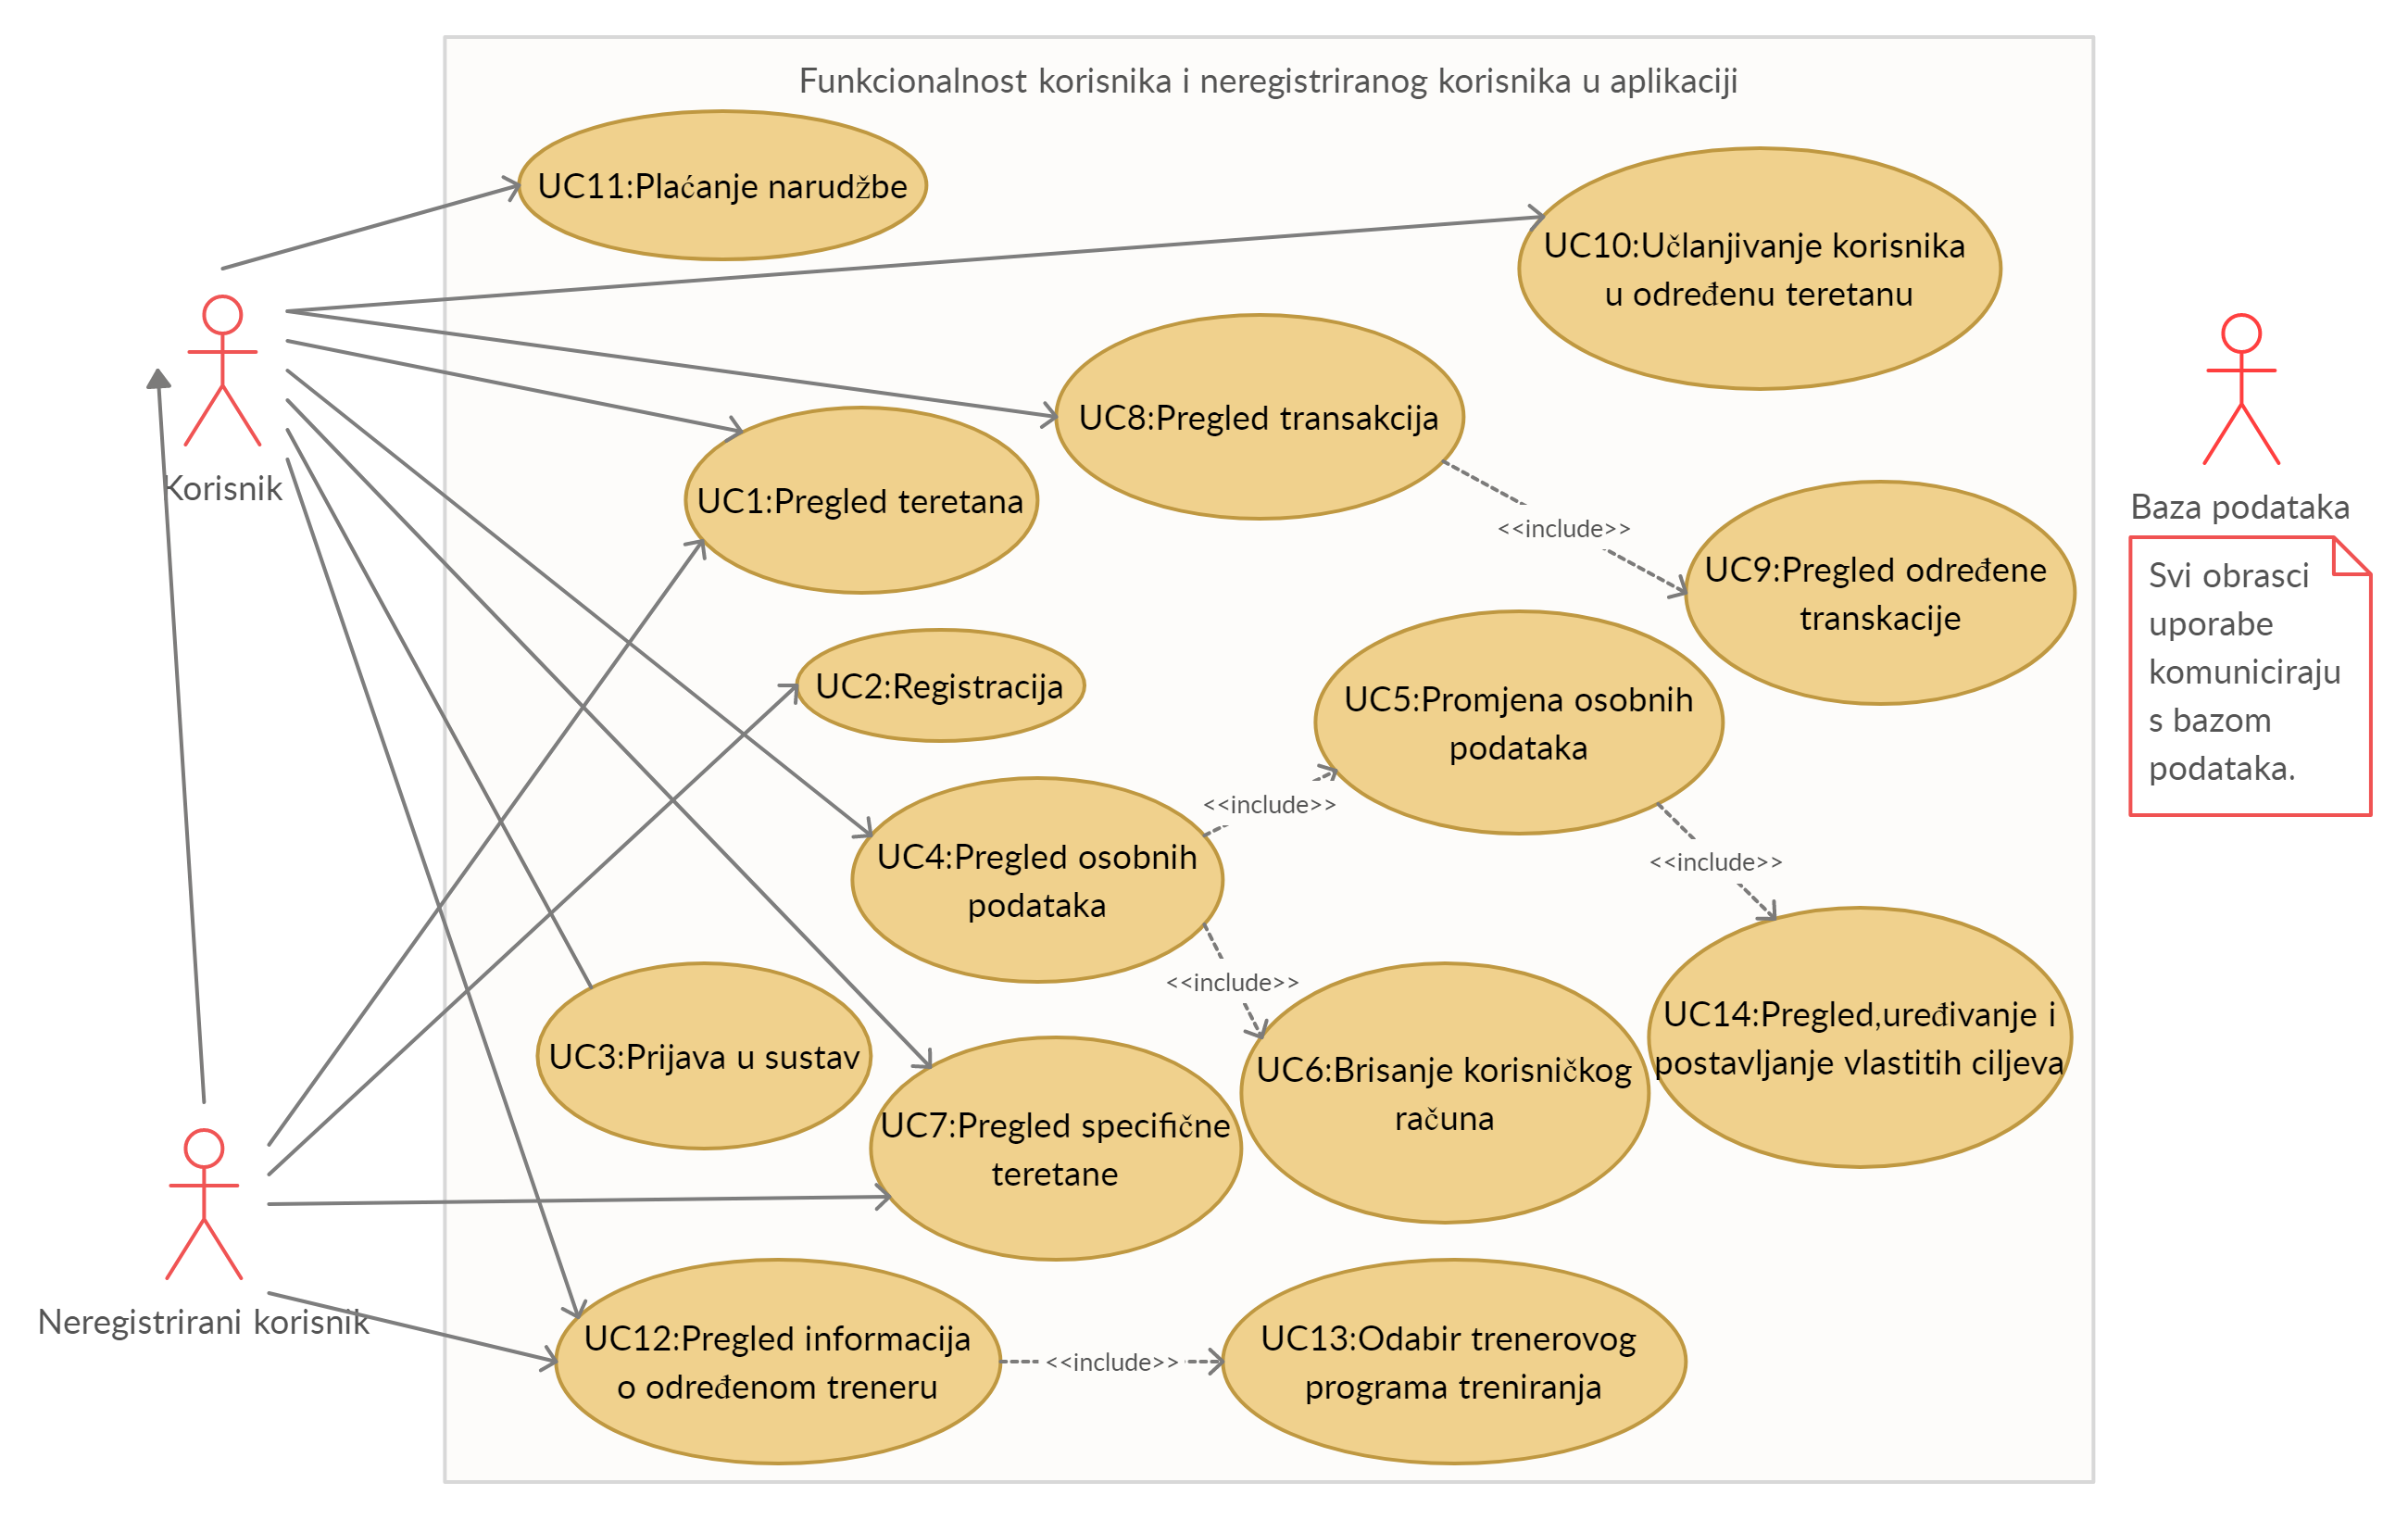
\includegraphics[height= 13cm,width=1.2\textwidth]{slike/obrazac1.jpg}
					\textbf{Slika 3.1: Dijagram obrasca uporabe, funkcionalnost korisnika i neregistriranog korisnika u aplikaciji  }

				\end{figure}
				
				\begin{figure}

    				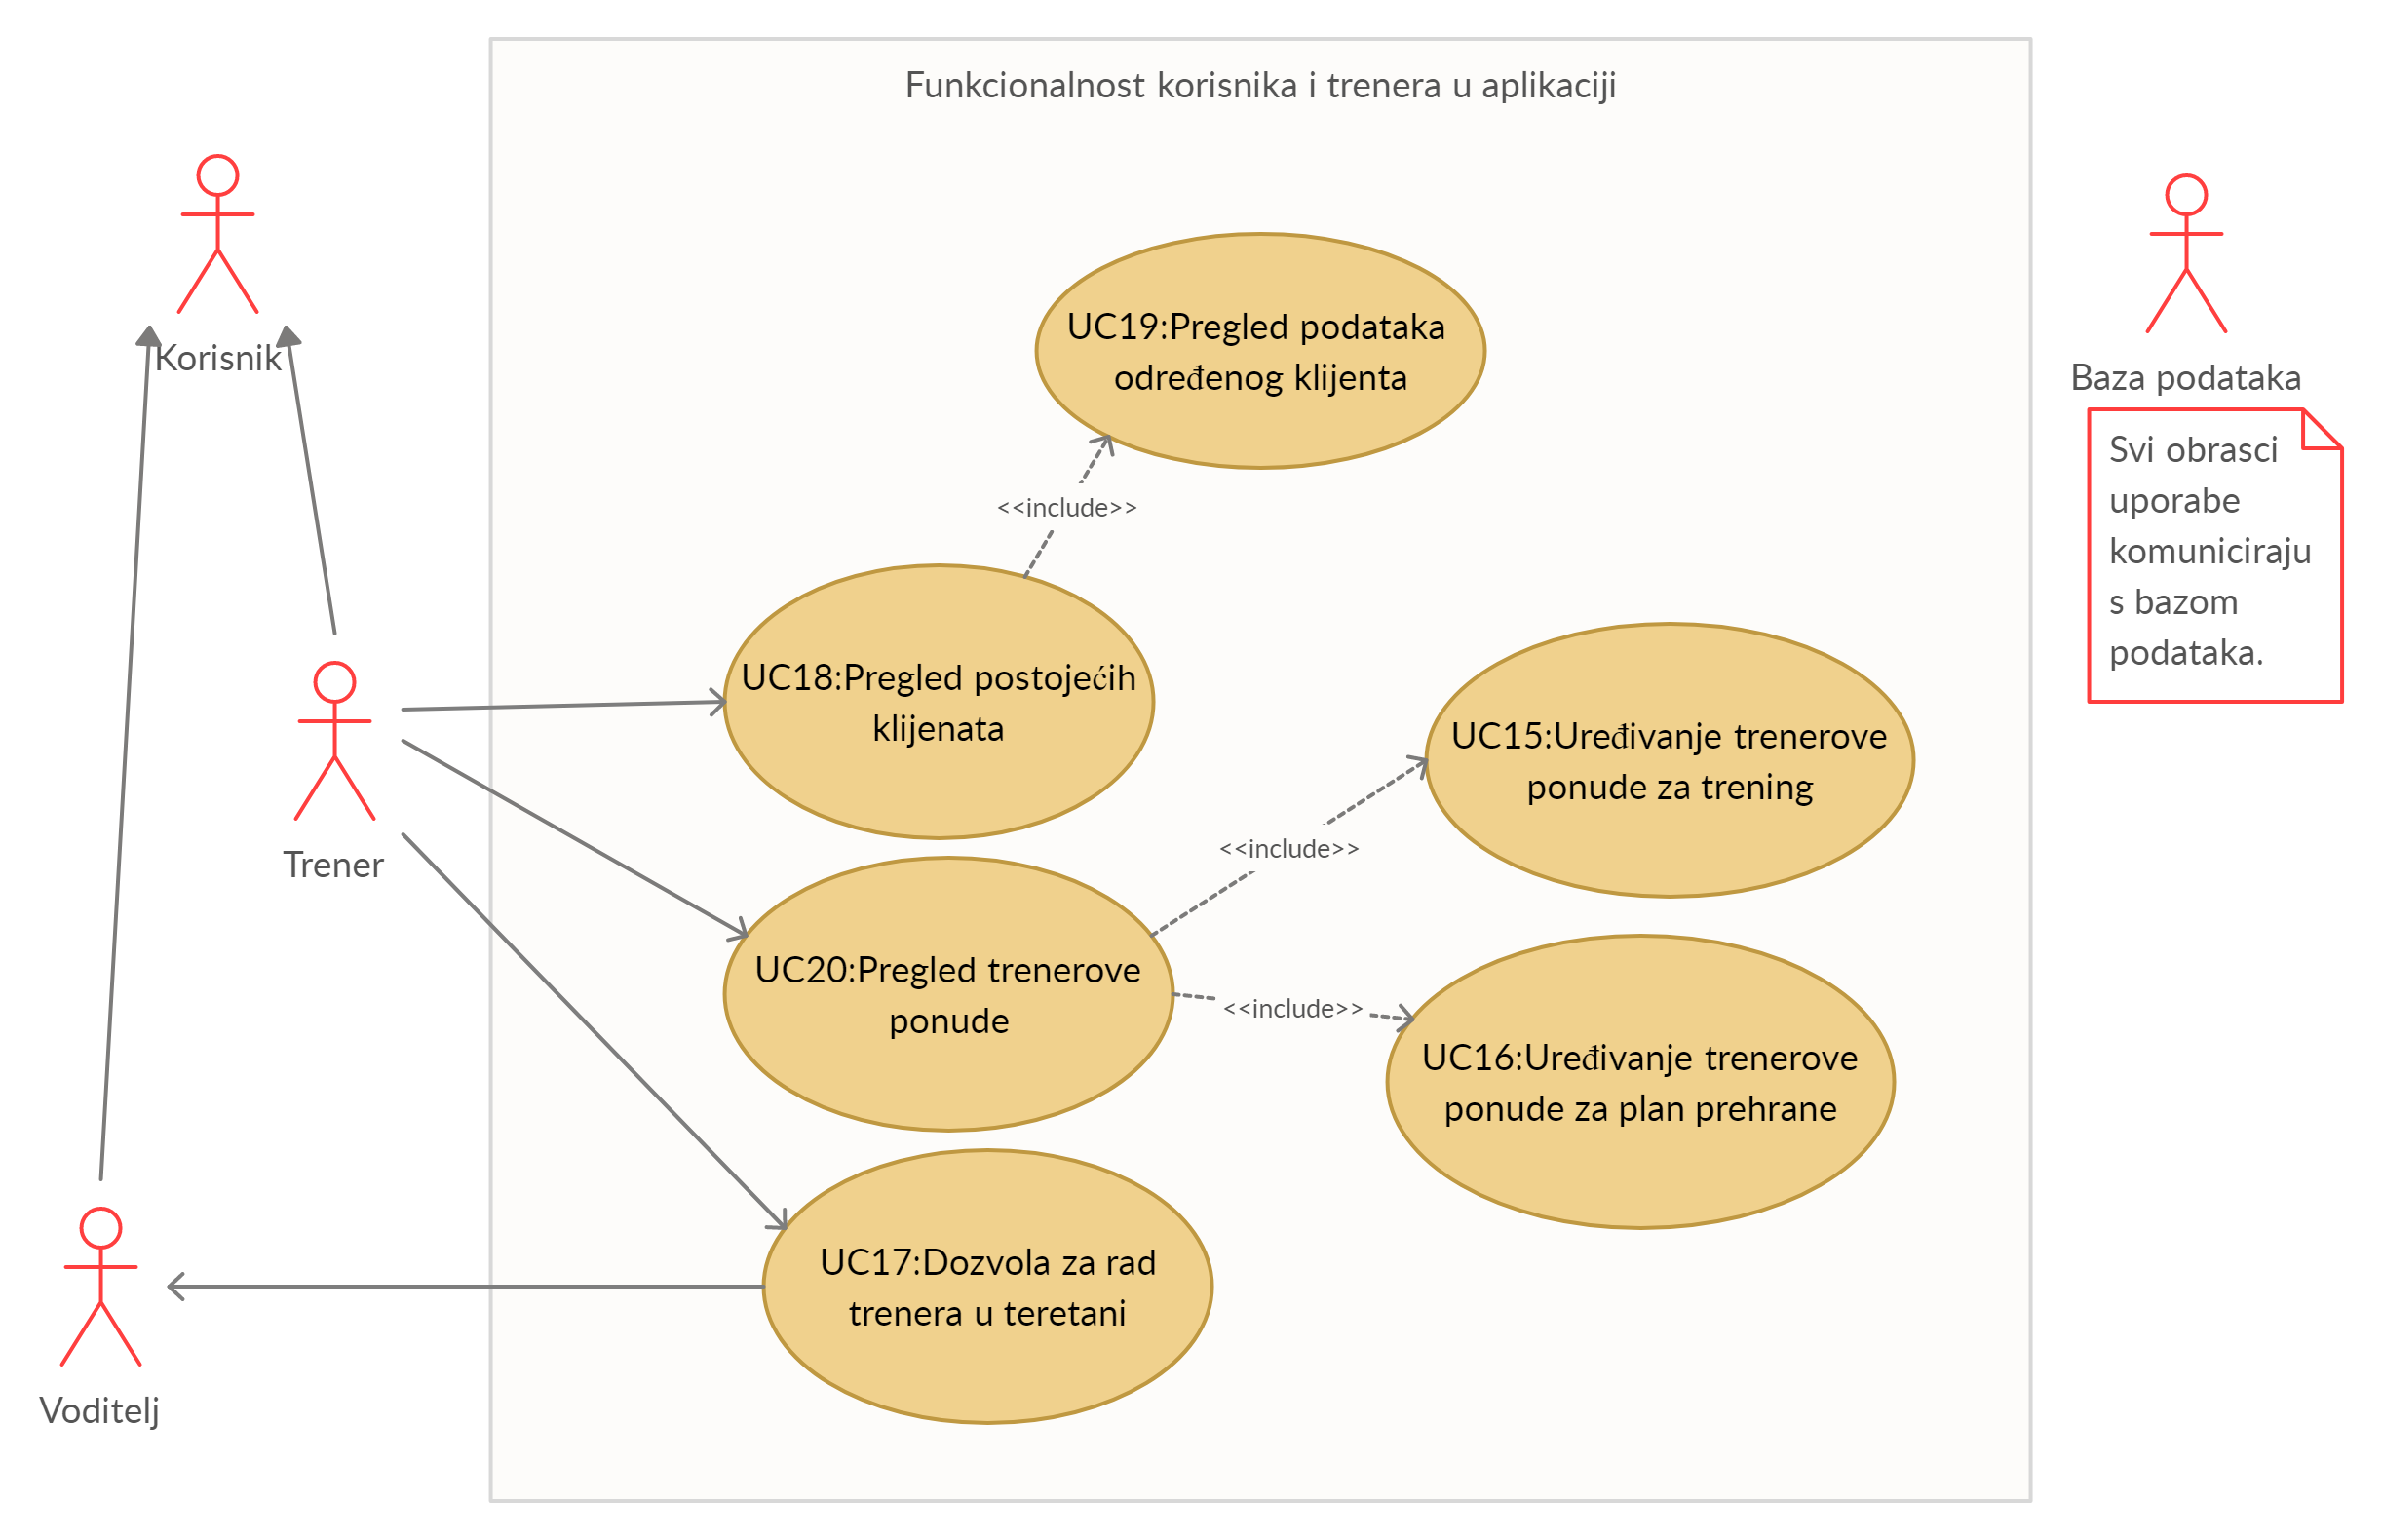
\includegraphics[height=13cm,width=1.2\textwidth]{slike/obrazac2.jpg}

    				\textbf{Slika 3.2: Dijagram obrasca uporabe, funkcionalnost korisnika i trenera u aplikaciji}
				\end{figure}
				
				\begin{figure}
    				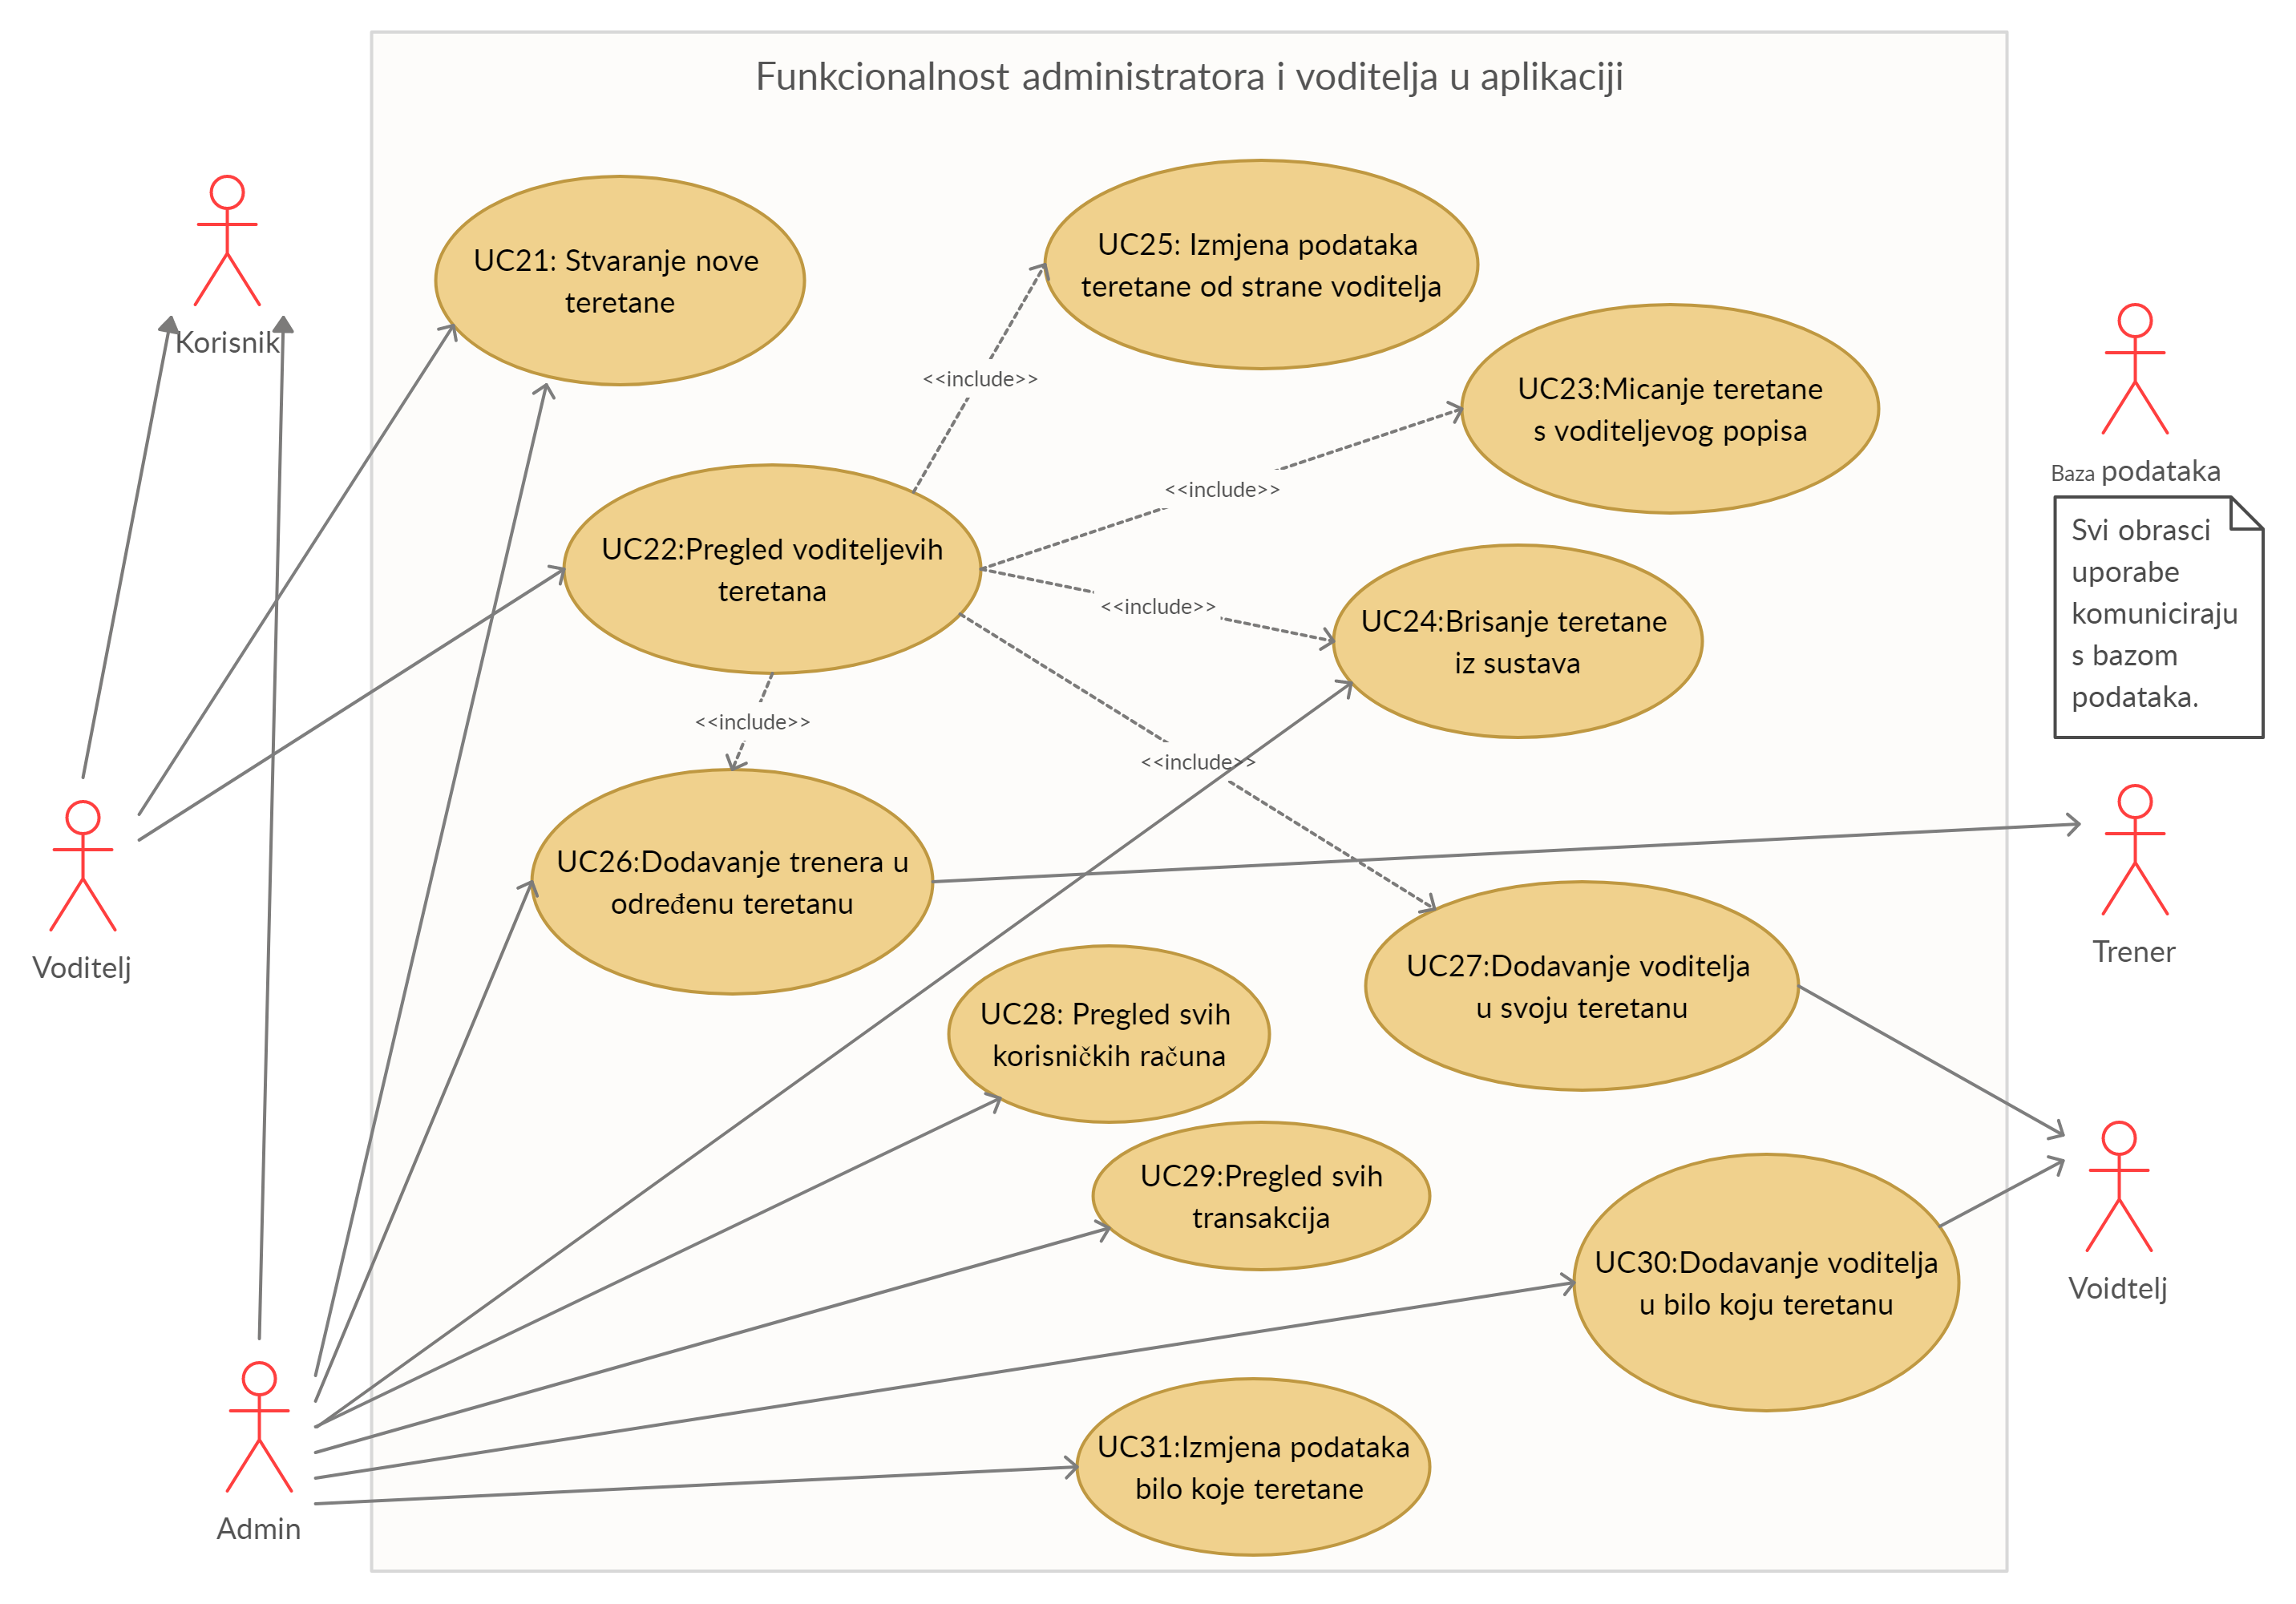
\includegraphics[height= 13cm,width=1.2\textwidth]{slike/obrazac3.jpg}
    				\textbf{Slika 3.3: Dijagram obrasca uporabe, Funkcionalnost korisnika i neregistriranog korisnika u aplikaciji}

				\end{figure}
			     
			       
			    \eject	
			 
			\subsection{Sekvencijski dijagrami}
				
				\textbf{\textit{dio 1. revizije}}\\
				
				\textit{Nacrtati sekvencijske dijagrame koji modeliraju najvažnije dijelove sustava (max. 4 dijagrama). Ukoliko postoji nedoumica oko odabira, razjasniti s asistentom. Uz svaki dijagram napisati detaljni opis dijagrama.}
				\eject
	
		\section{Ostali zahtjevi}
		
			\textbf{\textit{dio 1. revizije}}\\
		 
			 \textit{Nefunkcionalni zahtjevi i zahtjevi domene primjene dopunjuju funkcionalne zahtjeve. Oni opisuju \textbf{kako se sustav treba ponašati} i koja \textbf{ograničenja} treba poštivati (performanse, korisničko iskustvo, pouzdanost, standardi kvalitete, sigurnost...). Primjeri takvih zahtjeva u Vašem projektu mogu biti: podržani jezici korisničkog sučelja, vrijeme odziva, najveći mogući podržani broj korisnika, podržane web/mobilne platforme, razina zaštite (protokoli komunikacije, kriptiranje...)... Svaki takav zahtjev potrebno je navesti u jednoj ili dvije rečenice.}
			 
